\documentclass[a4paper,12pt]{report}

\usepackage[italian]{babel}
\usepackage[utf8]{inputenc}
\usepackage{amsmath}
\usepackage{parskip}
\usepackage{wrapfig}
\usepackage{graphicx}
\usepackage{subcaption}



\title{Robotic Sorter}
\author{Filippo Passarella, Ubaldo Tosi}

\begin{document}
\maketitle
\begin{center}
    Corso di studi di Ingegneria elettronica
\end{center}

\newpage
\section{Introduzione}
\section {Sensore di colore}
\begin{wrapfigure}{r}{0.3\textwidth}
    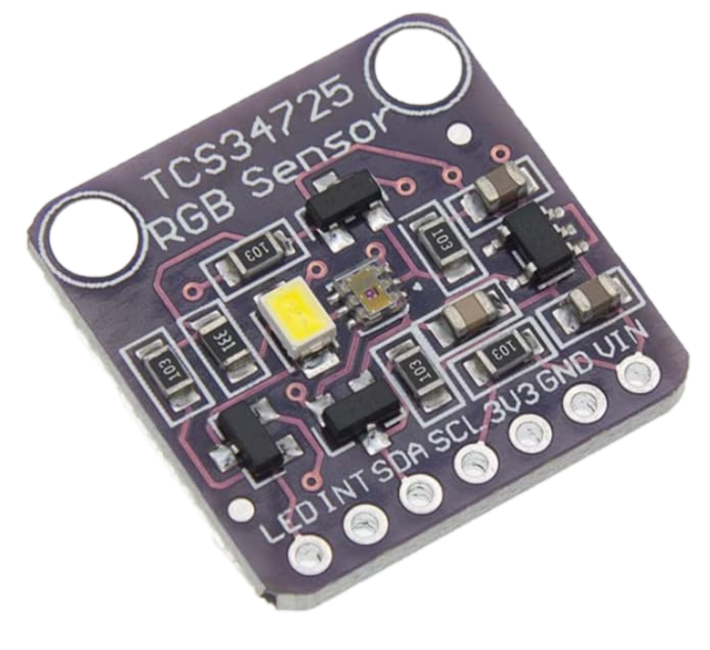
\includegraphics[width=0.8\linewidth]{images/Immagini sensore/pcb sensore.png}
    \caption{PCB Sensore}
\end{wrapfigure}
Il PCB del sensore di colore è costituito dal sensore di colore vero e proprio (TAOS TCS3472), un led bianco che permette di illuminare gli oggetti per misurare il colore della luce riflessa, spegnibile nel caso in cui si voglia misurare il colore di uno schermo o comunque qualcosa che emette luce propria, un regolatore $5V \rightarrow 3.3V$ che ci permette di alimentare il sensore a 5V e di usare la I2C a 5V per comunicare con il sensore grazie a due transistori messi come in figura. Inoltre integra le resistenze di pull-up.
\begin{figure}[h]
    \centering
    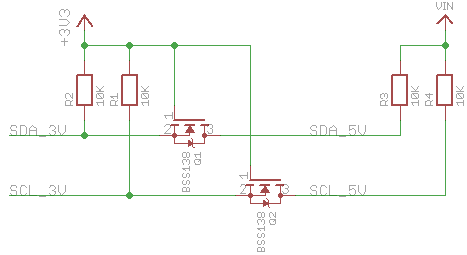
\includegraphics[width=0.35\linewidth]{images/Immagini sensore/I2C_3.3 to 5.png}
    \caption{I2C}
\end{figure}
\subsection{TAOS TCS3472}
\begin{figure}[h]
    \begin{subfigure}{0.5\textwidth}
    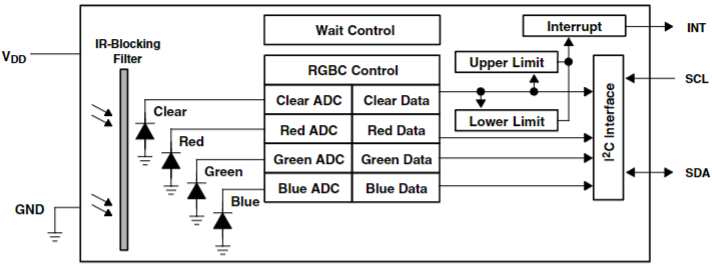
\includegraphics[width=0.8\linewidth]{images/Immagini sensore/Blocco funzionale.png}
    \caption{Blocco funzionale}
    \end{subfigure}
    \begin{subfigure}{0.4\textwidth}
    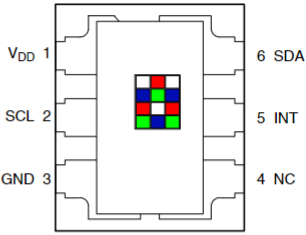
\includegraphics[width=0.4\textwidth]{images/Immagini sensore/sensore.png}
    \caption{Matrice fotodiodi sensore}
    \end{subfigure}
\end{figure}
Il sensore è costituito da una matrice 3x4 di fotodiodi con un filtro rosso, blu, verde e non filtrati (luce bianca), tutti i fotodiodi hanno un filtro ad infrarossi per aumentare l'accuratezza. La corrente generata da questi fotodiodi viene amplificata da un amplificatore trans-resistivo a guadagno variabile e campionata da un ADC integrativo a 16 bit per ogni colore. Il tempo di integrazione è programmabile. I dati poi vengono comunicati all'esterno attraverso l'interfaccia I2C (fino a 400 KHz). Il sensore può mandare un interrupt una volta che il valore del clear è sopra o sotto una certa threshold.
\begin{figure}[h]
    \centering
    \includegraphics[width=0.25\textwidth]{images/Immagini sensore/Responsività sensore.png}
    \caption{Responsività del sensore}
\end{figure}
Come si può vedere dall'immagine il sensore risponde molto bene al rosso e la responsività diminuisce andando verso il verde ed il blu questo come potremo vedere più avanti, unito al fatto che la luce del led tende al giallo porterà a problemi nella misura.
\subsubsection{I2C}
\begin{figure}[h]
    \centering
    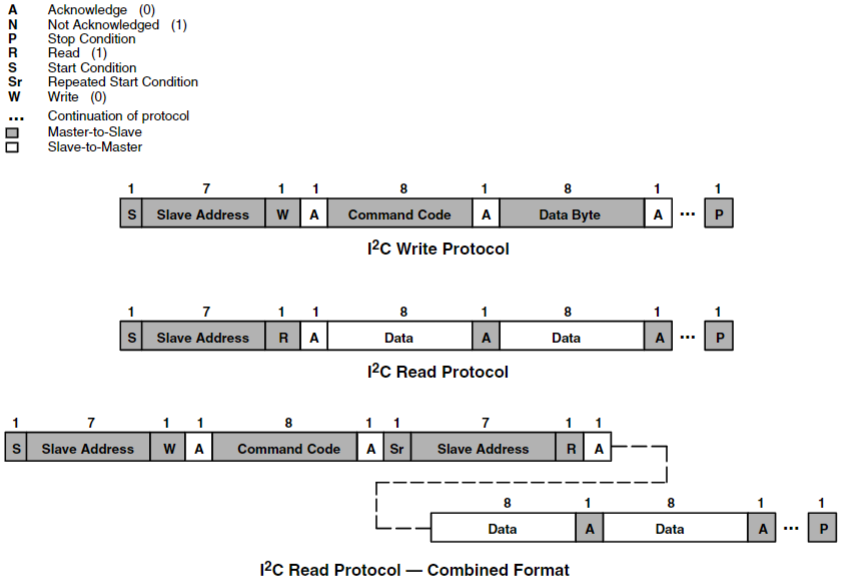
\includegraphics[width=0.70\textwidth]{images/Immagini sensore/I2C.png}
    \caption{I2C}
\end{figure}
Come possiamo vedere la scrittura dei registri mediante I2C viene fatta mandando per prima cosa lo start bit, poi l'indirizzo della periferica e il write. Una volta ricevuto l'acknowledge si manda il Command code. Questo configura il registro di Command.
\begin{figure}[h]
    \centering
    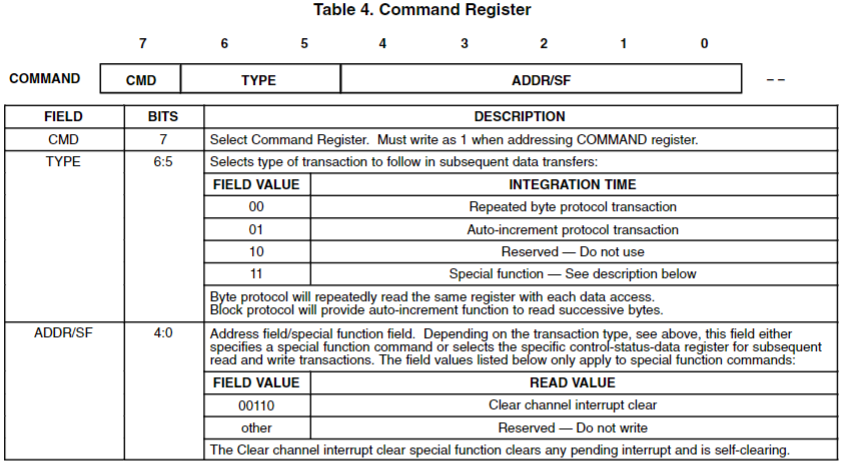
\includegraphics[width=0.7\textwidth]{images/Immagini sensore/registro di command.png}
    \caption{Registro Command}
    \label{fig:comm}
\end{figure}
Nel registro di Command possiamo stabilire se far leggere sempre lo stesso registro o scorrerli e da che indirizzo iniziare. Inoltre possiamo pulire gli interrupt.
Per la lettura una volta settato correttamente il registro command basta mandare lo start, l'indirizzo e il read e lui continuerà dopo ogni ack a mandare il dato successivo fino a che non riceve lo stop bit.
\subsubsection{Macchina a Stati sensore}
\begin{figure}[h]
    \centering
    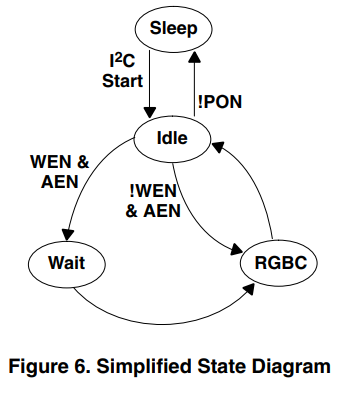
\includegraphics[width=0.35\textwidth]{images/Immagini sensore/macchina a stati.png}
    \caption{Macchina a stati}
\end{figure}
Il sensore per risparmiare energia rimane nello stato di sleep, una volta che riceve lo start dall'I2C va in idle ed in base a se è settato il bit di wait o meno fa subito la misura oppure aspetta un certo tempo. Una volta fatta la misura torna in idle e in caso di power on disabilitato torna in sleep. La macchina a stati dipende principalmente dai parametri del registro Enable (0x00).
\clearpage
\subsubsection{Registri}
\begin{figure}[h]
    \centering
    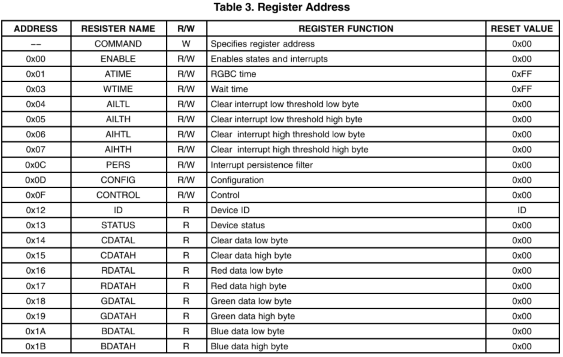
\includegraphics[width=0.5\textwidth]{images/Immagini sensore/Indirizzi sensore.png}
    \caption{Registri sensore}
\end{figure} 
\subsubsection{Parametri scelti}
\label{subsec:Parametri sensore}
\begin{table}[h]
    \centering
    \begin{tabular}{ccc}
        Indirizzo & Nome & Valore \\
        ---- & Command & 10100000 \\
        0x00 & Enable & 0x03 \\
        0x01 & Timing & 0xC0 \\
        0x0F & Control & 0x03
    \end{tabular}
    \caption{Indirizzi settati}
    \label{tab:my_label}
\end{table}
Solo questi registri sono stati settati in quanto si è scelto di non utilizzare l'interrupt per decidere quando leggere il sensore, ma piuttosto di fare un polling alla pressione di un pulsante ed eseguire a quel punto 3 misure così da implementare un voter. Questo perché i livelli di luminosità registrati dal sensore erano simili tra con il cubetto sopra e senza e variavano più in base al colore del cubetto che dal fatto che fosse sopra o no.

\subsubsection{Command}
Come visibile nella figura \ref{fig:comm} per fare la lettura e scrittura abbiamo deciso di usare registro di Enable come primo registro e di fare le letture sequenziali degli indirizzi.
\clearpage
\subsubsection{Enable}
\begin{figure}[h] 
    \centering
    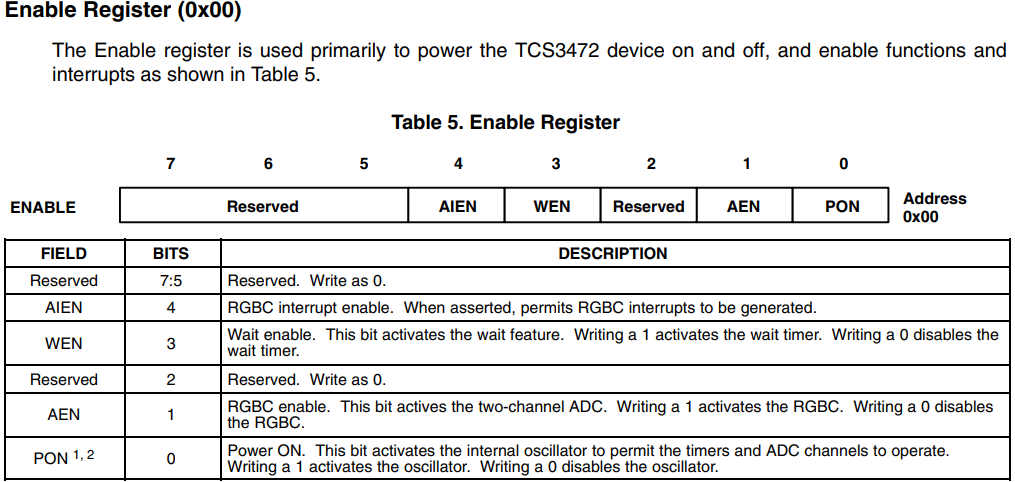
\includegraphics[width=0.65\linewidth]{images/Immagini sensore/registro enable.png}
    \caption{Enable Register}
\end{figure}
Come scritto nella sezione \ref{subsec:Parametri sensore} abbiamo ovviamente attivato il power on e gli ADC mentre non abbiamo attivato gli interrupt e il wait.
Non è stato attivato il wait in quanto per la nostra applicazione abbiamo preferito dare priorità alla velocità di lettura che al power management tenendo anche conto che si fanno 3 letture del sensore ogni volta.
\subsubsection{Timing e Control}
\begin{figure}[h] 
    \centering
    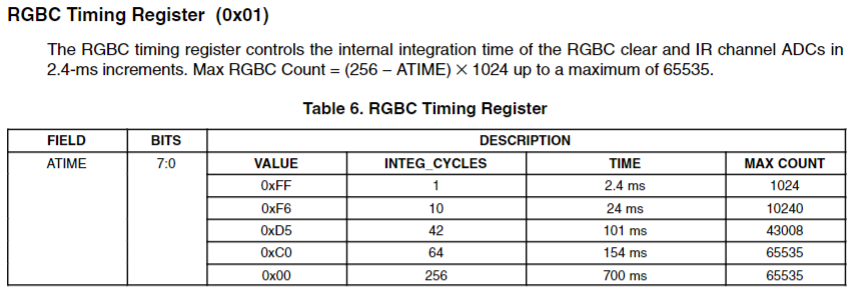
\includegraphics[width=0.65\linewidth]{images/Immagini sensore/registro timing.png}
    \caption{Registro timing}
    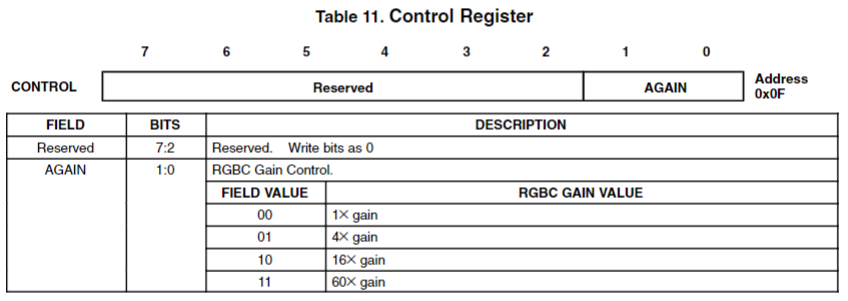
\includegraphics[width=0.65\linewidth]{images/Immagini sensore/registro control.png}
    \caption{Registro control}
    \end{figure}
    I valori dei registri di timing e control sono stati scelti in tandem in quanto sono i valori che influenzano la lettura e la sua accuratezza. Il registro di timing modifica il tempo di integrazione degli ADC e quindi influisce sulla sensibilità e sulla risoluzione della misura mentre quello di control determina il guadagno dell'amplificatore. Inizialmente per il timing ci siamo imposti un tempo massimo per le 3 misure di 1,5 secondi. Sapendo che $Timing = (0xFF - 0xATIME) * 2.4ms$ Possiamo calcolare il \(ATIME_{min} = 0x2A\). Inizialmente abbiamo provato con il massimo guadagno (x60) e abbiamo aumentato il tempo di integrazione fino a raggiungere dei valori con un buon valore massimo e minimo con tutti i colori evitando la saturazione ovvero \(ATIME_{1} = 0xC0\) ovvero Timing = 154ms così da avere un buon compromesso tra il tempo di integrazione e la risoluzione e sensibilità dei valori misurati. Successivamente abbiamo fatto una prova usando il massimo tempo di integrazione considerato accettabile (\(ATIME_{2} = 0x2A\)  ovvero Timing = 510ms) ed aumentato il guadagno fino ad arrivare ad un valore né troppo basso né in saturazione per ogni colore, ovvero (x16).
    \label{subsubsec:Timing}
    \begin{table}[h]
        \centering
        \begin{tabular}{ccc}
            Registro & Configurazione 1 & Configurazione 2\\
             Timing& 0xC0 & 0x2A\\
             Control& 0x03 & 0x02\\
        \end{tabular}
        \caption{Configurazioni}
        \label{tab:configurazioni}
    \end{table}
    \begin{table}[h]
        \centering
        \begin{tabular}{ccc}
            Registro & Configurazione 1 & Configurazione 2\\
             $Red_L$& 01 & 6A\\
             $Red_H$& FF & D6\\
             $Green_L$& 31 & E4\\
             $Green_H$& 2F & 26\\
             $Blue_L$& 62 & 97\\
             $Blue_H$& 25 & 1F\\
        \end{tabular}
        \caption{Cubo rosso}
        \label{tab:cubo_rosso}
    \end{table}
    \begin{table}[h]
        \centering
        \begin{tabular}{ccc}
            Registro & Configurazione 1 & Configurazione 2\\
             $Red_L$& 2D & E4\\
             $Red_H$& 49 & 43\\
             $Green_L$& 03 & 2B\\
             $Green_H$& 80 & 79\\
             $Blue_L$& 77 & F4\\
             $Blue_H$& 6C & 66
        \end{tabular}
        \caption{Cubo blu}
        \label{tab:cubo_blu}
        \end{table}
        \begin{table}[h]
        \centering
        \begin{tabular}{ccc}
            Registro & Configurazione 1 & Configurazione 2\\
             $Red_L$& 79 & 48\\
             $Red_H$& 5A & 55\\
             $Green_L$& CD & 89\\
             $Green_H$& 80 & 7C\\
             $Blue_L$& 9A & 6C\\
             $Blue_H$& 3D & 38
        \end{tabular}
        \caption{Cubo verde}
        \label{tab:cubo_verde}
    \end{table}
Vedendo che la differenza tra le due configurazioni era trascurabile si è optato per l'uso della prima così da risparmiare un secondo nella misura.
Un problema riscontrato è stato quello della misura sul cubo blu in quanto il colore dal valore più alto è risultato il verde ed il blu solo il secondo più alto. Provando a cambiare colore con un cartoncino più scuro il colore con il valore più alto risultava invece il rosso a causa del grande assorbimento di luce del cartoncino blu scuro. Questo è dovuto in parte al fatto che la luce del led in dotazione tende un po' verso il giallo (componente rossa più accentuata) e alla maggior responsività alla luce rossa e verde rispetto alla blu.
\subsection{Lettura}
\begin{figure}[h] 
    \centering
    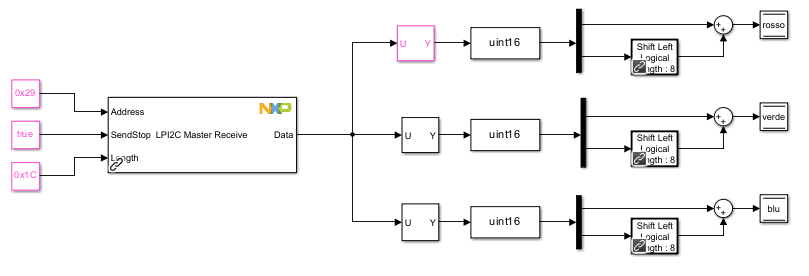
\includegraphics[width=0.76\linewidth]{images/Immagini sensore/lettura sensore.png}
    \caption{lettura sensore}
    \end{figure}
\begin{figure}[h]
    \centering
    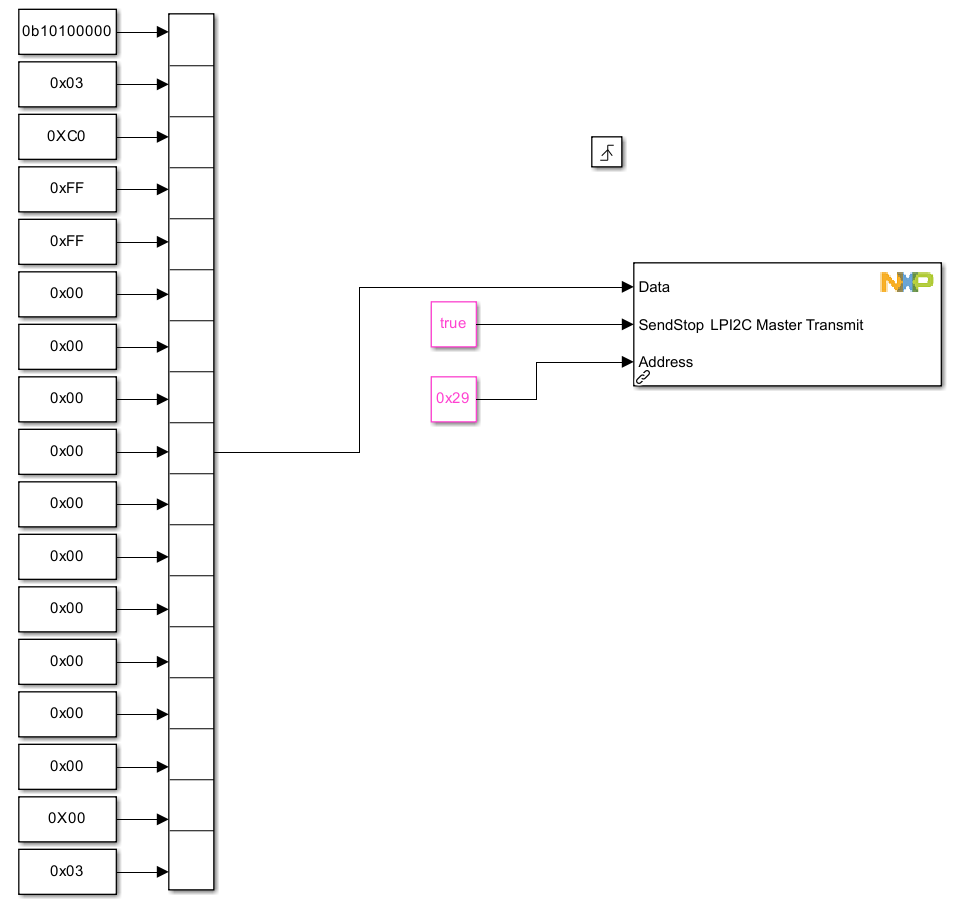
\includegraphics[width=0.6\linewidth]{images/Immagini sensore/scrittura sensore.png}
    \caption{scrittura sensore}
    \end{figure}
Si è deciso di leggere tutti i blocchi ogni volta che fosse stata necessaria la lettura per evitare dopo la scrittura di dover riscrivere il registro command con il nuovo indirizzo di partenza visto che il guadagno in termini di tempo era trascurabile. Una volta eseguita la lettura di esegue la somma pesata dei valori h e l dei registri di ogni colore per avere il valore effettivo a 16 bit.
\subsection{Macchina a stati}
\begin{figure}[h] 
    \centering
    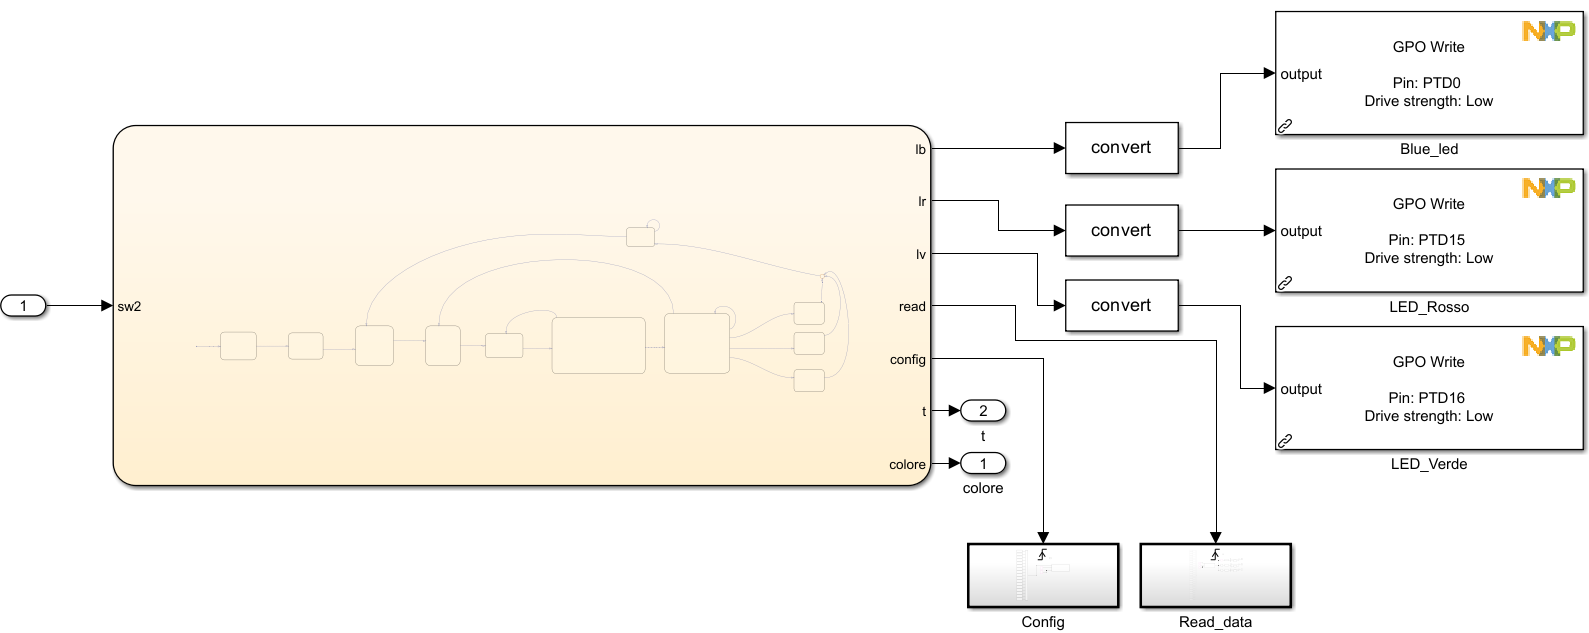
\includegraphics[width=0.6\linewidth]{images/Immagini sensore/Sensing e macchina a stati.png}
    \caption{Matlab sensing}
    \end{figure}
\begin{figure}[h]
    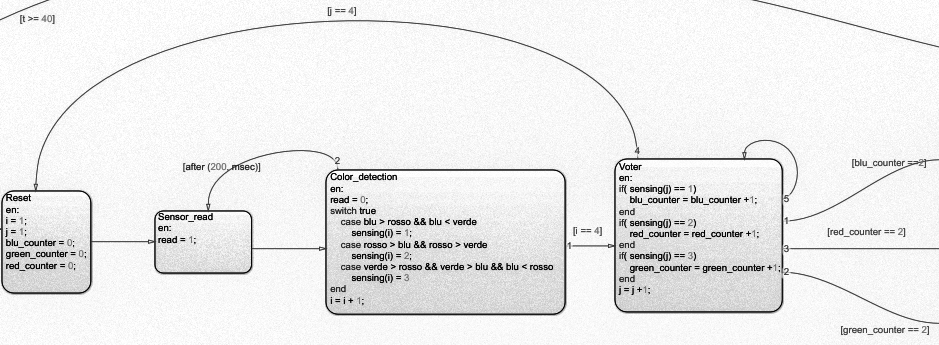
\includegraphics[width=0.8\linewidth]{images/Immagini sensore/sensor_chart.png}
    \caption{Macchina a stati}
    \label{fig:stateflow}
\end{figure}
Come possiamo vedere nella figura \ref{fig:stateflow} all'accensione viene configurato il sensore e messo colore a 4 per mettere il braccio ad una posizione di default Successivamente si entra in uno stato di wait in cui si resettano tutti i contatori. Premendo il pulsante sw2 si passa allo stato di reset del voter. Successivamente si eseguono 3 letture con conseguente decisione del colore per ogni misura. A quel punto il voter decide il colore del cubo se vi sono 2 colori uguali oppure rifà le misure se sono tutti e 3 diversi. Per finire incrementa un contatore ogni 200ms per fare l'attuazione.
\subsubsection{Voter}
\begin{figure}[h] 
    \centering
    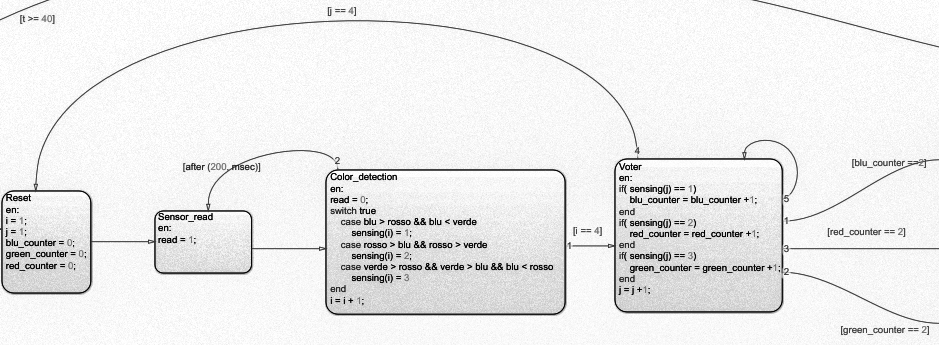
\includegraphics[width=0.75\linewidth]{images/Immagini sensore/voter.png}
    \caption{Voter}
\end{figure}
Per stabilire con accuratezza il colore del cubo è stato necessario implementare un voter in quanto durante i test la misura a volte risultava diversa per cui si è deciso di applicare una ridondanza nelle misure a scapito della velocità di misura. Perle ragioni esposte nella sezione \ref{subsubsec:Timing} nel blocco color detection è stato necessario per il riconoscimento del blu mettere che blu fosse compreso tra il verde e il rosso.
\subsection{Test}
Purtroppo non è stato possibile fare il PIL dei blocchi contenenti la comunicazione via I2C in quanto Matlab dava errore in caso di presenza dei blocchi di send e receive via I2C.
\begin{figure}[h] 
    \centering
    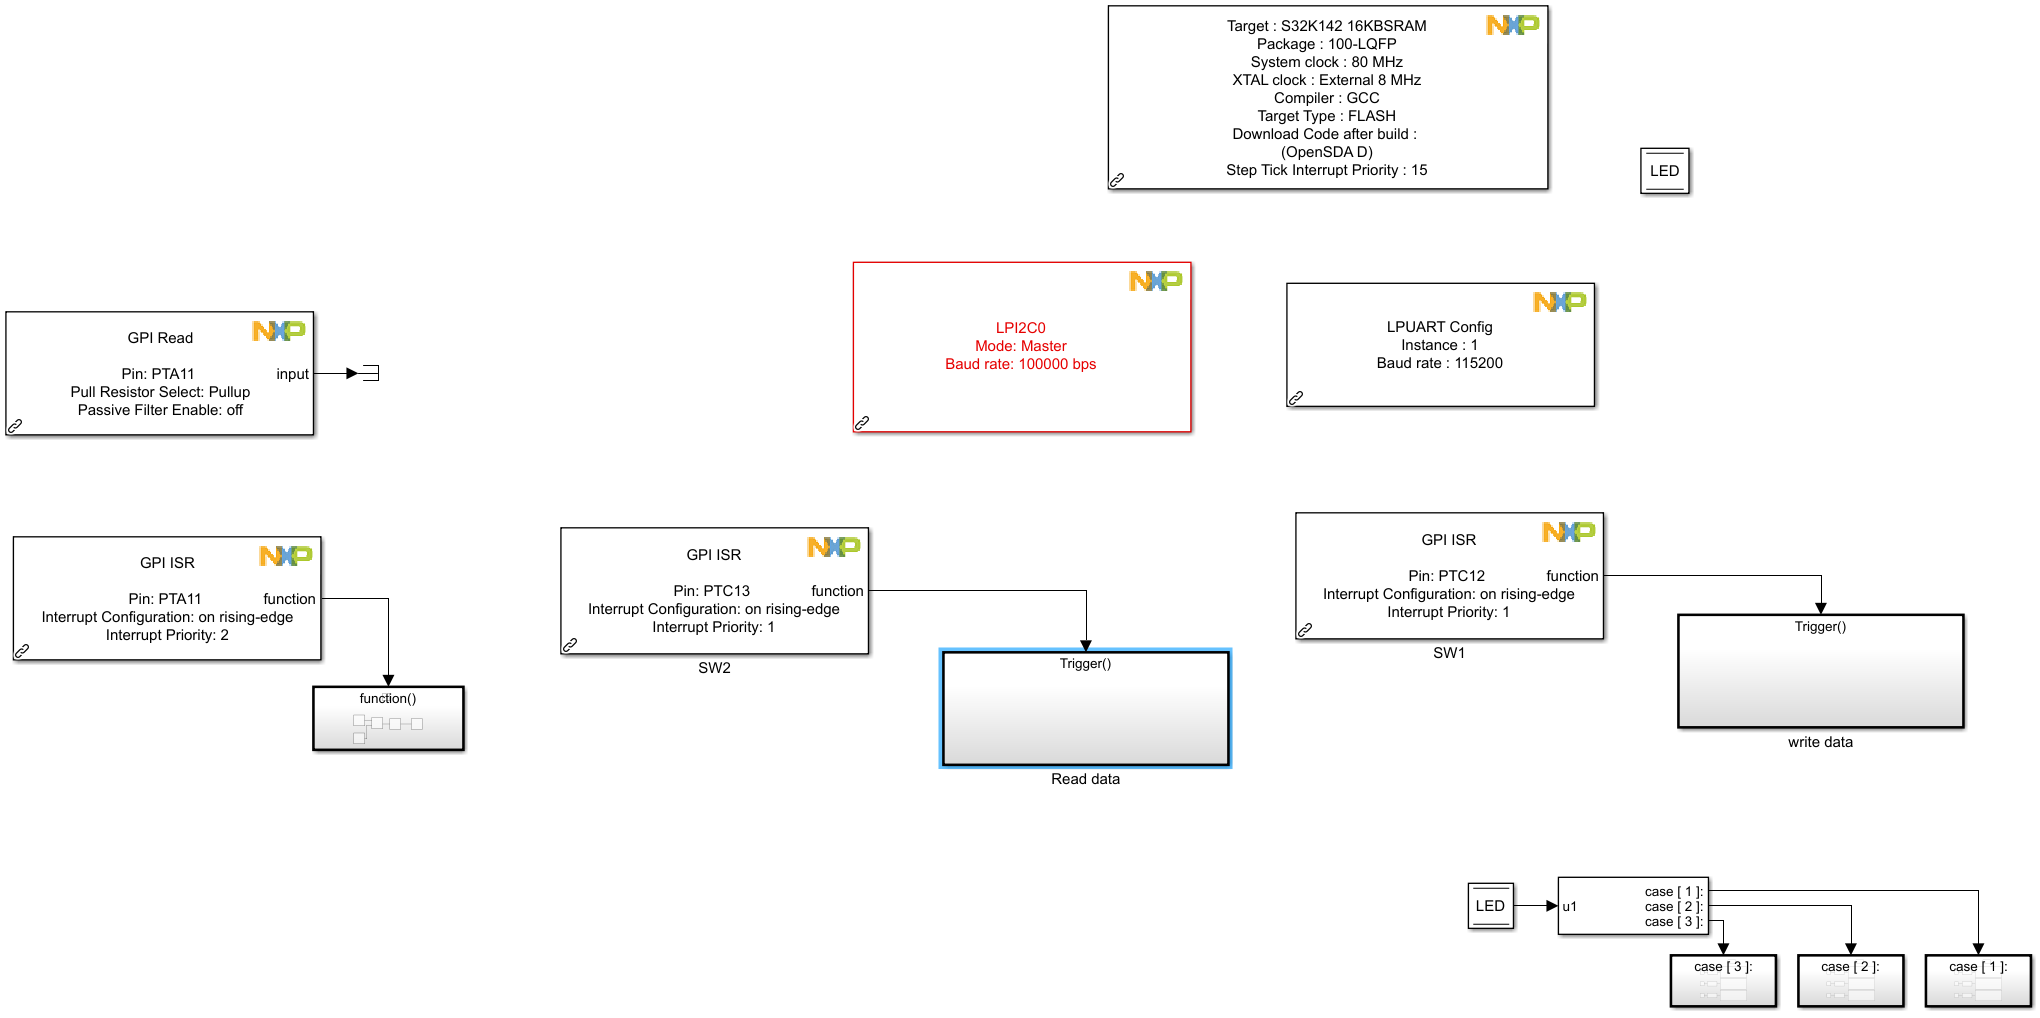
\includegraphics[width=0.6\linewidth]{images/Immagini sensore/i2c_test.png}
    \caption{Test I2C}
\end{figure}
Per eseguire i test della parte di sensore inizialmente è stato fatto un file Matlab che si occupava solo di comunicare con il sensore e mandare i dati ricevuti via uart al pc così da poter valutare i parametri migliori per il sensore.
Una volta individuati è stata fatta la macchina a stati e testata prima in MIL e poi usando la uart e il led rgb per il debug.
\begin{figure}[h] 
    \centering
    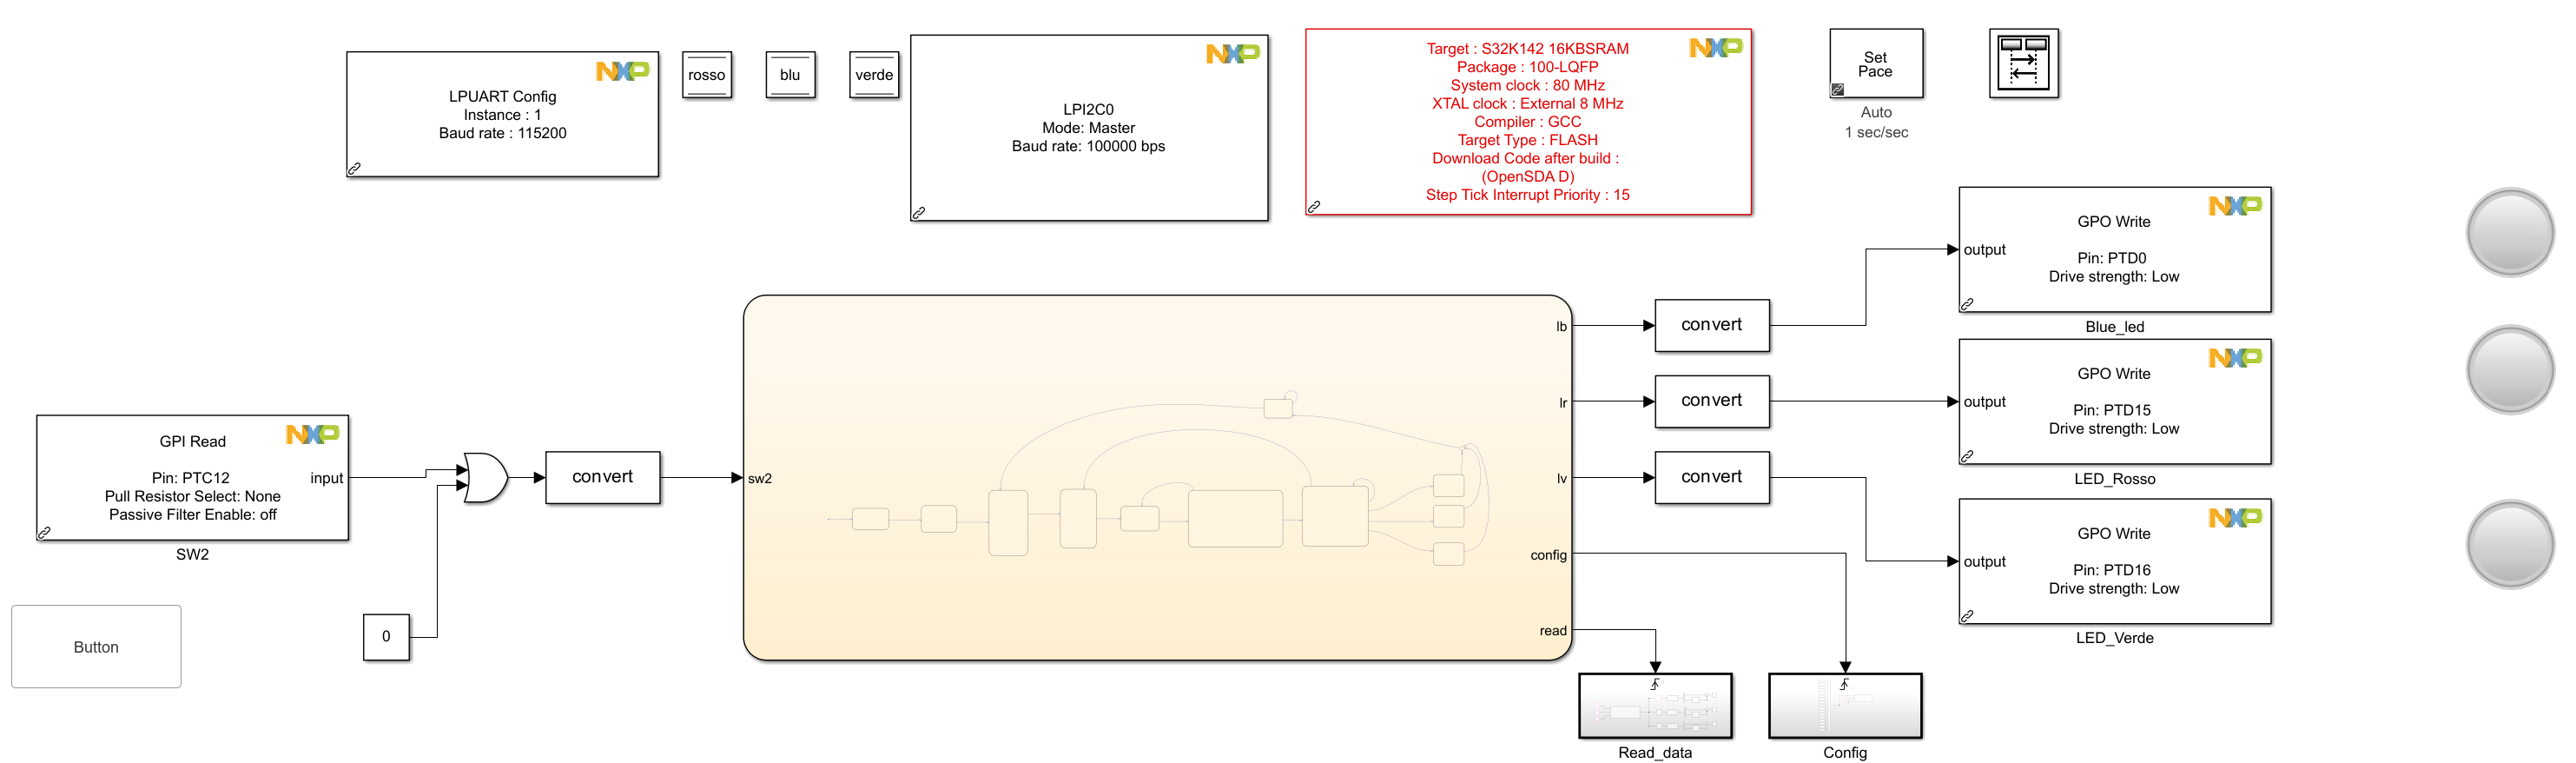
\includegraphics[width=0.75\linewidth]{images/Immagini sensore/test_stateflow_2.png}
    \caption{Test macchina a stati}
\end{figure}
Una volta controllato che tutto funzionasse a dovere è stato unito alla parte di attuazione ed è stato testato il tutto prima in modalità MIL e poi usando la uart per il debug. Una volta risolti eventuali problemi abbiamo attaccato il braccio e testato il comportamento fisico ottimizzando i path.
\begin{figure}[h] 
    \centering
    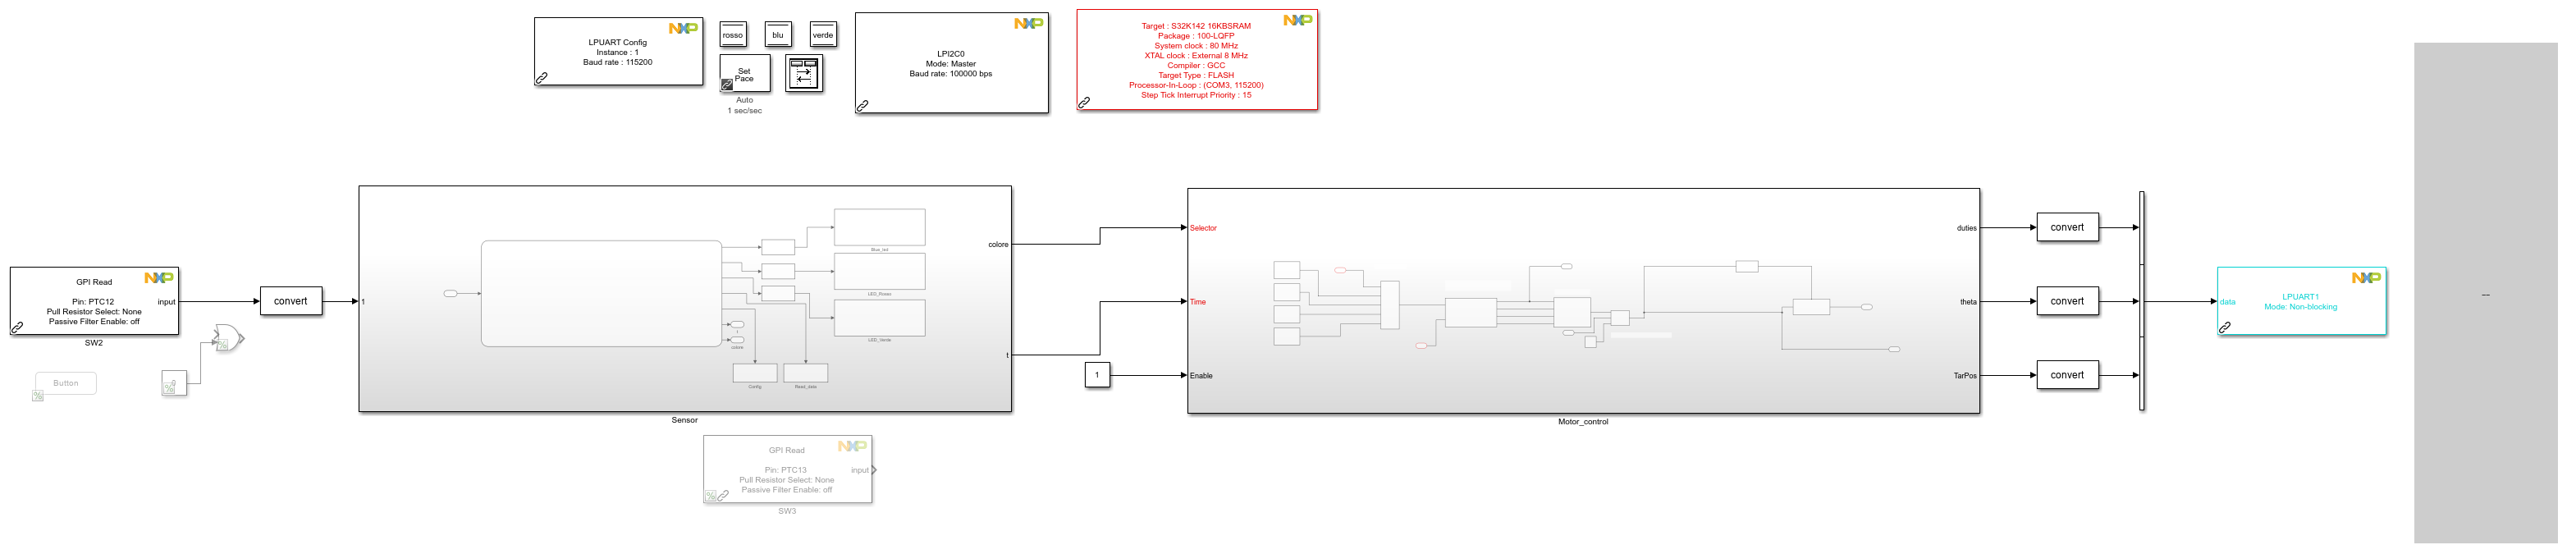
\includegraphics[width=0.75\linewidth]{images/Immagini sensore/Matlab_completo.png}
    \caption{MIL completo}
\end{figure}
\subsection{Miglioramenti}
\begin{enumerate}
    \item Trovare cartoncini blu tali per cui il valore del blu il maggiore rispetto agli altri
    \item Spegnere il led del sensore quando non si sta facendo la misura per ridurre il consumo di energia
\end{enumerate}
\section{Controllo motori}
\section{Conclusioni}
\end{document}
